\documentclass[12pt]{article}  

\usepackage[boxruled,lined]{algorithm2e}
%% \usepackage{booktabs}
\usepackage{amsmath} 
\usepackage{amsthm} 
\usepackage{amsfonts} 
\usepackage{enumitem}
\usepackage[T1]{fontenc}
\usepackage{xparse} 
\usepackage{bm}
\usepackage{bbm} 
\usepackage{color,soul} 
\usepackage{framed}
\usepackage[margin=0.5in]{geometry}
\usepackage{hyperref}
\usepackage{mathtools}
\usepackage{multicol}
\usepackage[dvipsnames]{xcolor}
\usepackage{tikz}
\usepackage[normalem]{ulem}
\usepackage{pgfplots}  
\usepackage{pifont}
\usetikzlibrary{positioning}
\usetikzlibrary{calc}
\usetikzlibrary{fit}
\usetikzlibrary{shapes}
\usetikzlibrary{patterns}
\usetikzlibrary{decorations.pathreplacing}
\newcommand\STAR{{\tikz{\node[draw,star,star point height=.7em,minimum size=1em,scale=0.35]{};} }}
\newcommand{\Plus}{\mathord{\begin{tikzpicture}[baseline=0ex, line width=1, scale=0.13]
\draw (1,0) -- (1,2); \draw (0,1) -- (2,1); \end{tikzpicture}}}

\newtheorem{theorem}{Theorem}[section]
\newtheorem{lemma}[theorem]{Lemma}
\newtheorem{proposition}[theorem]{Proposition}
\newtheorem{corollary}[theorem]{Corollary}
\DeclarePairedDelimiter{\ceil}{\lceil}{\rceil}
\DeclarePairedDelimiter{\floor}{\lfloor}{\rfloor}
\DeclareMathOperator*{\argmin}{arg\,min}
\DeclareMathOperator*{\argmax}{arg\,max}
\newcommand{\D}{\mathrm{d}}
\SetKwInput{KwInput}{Input}
\SetKwInput{KwOutput}{Output}

\begin{document}
\renewcommand{\d}[1]{\ensuremath{\operatorname{d}\!{#1}}}

\tableofcontents
\newpage
\section{Classification and Vector Spaces}\vspace{.1pt} \hrule height 2pt \smallskip \renewcommand{\arraystretch}{1}% Tighter
\subsection{Supervised ML and Sentiment Analysis}
In supervised ML, we have input features $X$ and a set of labels $Y$. To get the most accurate predictions, we try to minimize our \emph{error rates} or \emph{cost function} as much as possible: to do this, we'll run our prediction function which takes in parameters $\theta$ to map you input features to output labels $\hat Y$. The best mapping is achieved when the difference between the expected values $Y$ and the predicted values $\hat Y$ is minimized, which the cost function does by comparing how closely your output $\hat Y$ is to your label $Y$. You can then update your parameters and repeat the whole process until your cost is minimized.

\begin{center}
  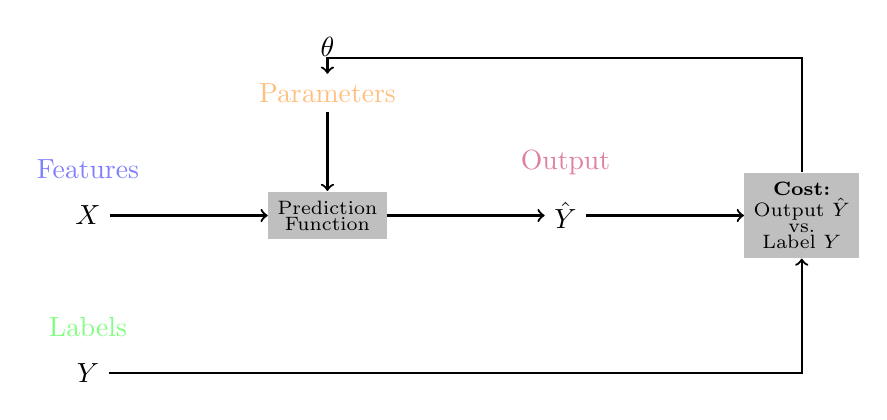
\begin{tikzpicture}
    \node (x) at (0, 2) {$X$};
    \node (features) [above=1mm of x] {\color{blue!50}{Features}};
    \node (y) at (0, 0) {$Y$};
    \node (labels) [above=1mm of y] {\color{green!50}{Labels}};
    \node[fill=gray!50,rectangle,right = 2cm of x] (predictionfunction)     {$\substack{\textrm{Prediction} \\ \textrm{Function}}$};
    \node[above = 1cm of predictionfunction] (params)     {\color{orange!50}{Parameters}};
    \node[above = 1mm of params] (theta) {$\theta$};
    \node[right = 2cm of predictionfunction] (yhat) {$\hat Y$};
    \node (output) [above=1mm of yhat] {\color{purple!50}{Output}};
    \node[fill=gray!50,rectangle,right = 2cm of yhat] (cost) {$\substack{\textrm{\textbf{Cost:}} \\ \textrm{Output } \hat Y \\ \textrm{vs.}     \\ \textrm{Label } Y}$};
\draw[->,thick] (x) -- (predictionfunction);
\draw[->,thick] (predictionfunction) -- (yhat);
\draw[->,thick] (yhat) -- (cost);
% Draw a path in two steps and go via a coordinate relative to the first node.
\draw[->,thick] (y) -- node {} ++(2cm,0) -| (cost);
\draw[->,thick] (cost) -- node{} ++(0,2cm) -| (params);
\draw[->,thick] (params) -- (predictionfunction);
  \end{tikzpicture}
\end{center}

How about the supervised ML classification task of sentiment analysis? Suppose we're given a tweet that says, ``I'm happy because I'm learning NLP'': and the objective in the task is to predict whether a tweet has a positive or negative sentiment. We'll do this by starting with a training set where tweets with a positive label have a label of unit value, and tweets with a negative sentiment have a label of zero.
To get started building a logistic regression classifier that's capable of predicting sentiments of an arbitrary tweet, we first need to process the raw tweets in our training data set and extract useful features. Then, we will train our logistic regression classifier while minimimizing the cost. Finally, we'll be able to make predictions.

\paragraph{How to represent text as a vector} In order to represent text as a vector, we need to first build a vocabulary. We define the vocabulary $V$ as the \emph{set} of unique words from your input data (e.g. your listing of tweets). To get this listing, we quite literally need to comb through all words from all input data and save every new word that appears in our search.
To represent a tweet as a vector, we can use a one-hot encoding with our vocabulary: i.e. each tweet will be represented with a length $|V|$ vector where elements are binary-valued - a one indicates the word is in the tweet and a zero indicates the absence of a word in a tweet. We call this a \emph{sparse} representation because the number of non-zero entries is relatively small when compared with the number of zero entries. Realize that if we are running a logistic regression, we would require learning $|V| + 1$ parameters which can be problematic for large vocabularies. If not prohibitive, it would make training models take excessive time and making predictions would be expensive.

\paragraph{Negative and positive frequencies}


\end{document}
